\subsection{Semantics of CTL}


\begin{frame}{Semantics}
    \framesubtitle{Intuition of semantics}
    \begin{figure}
        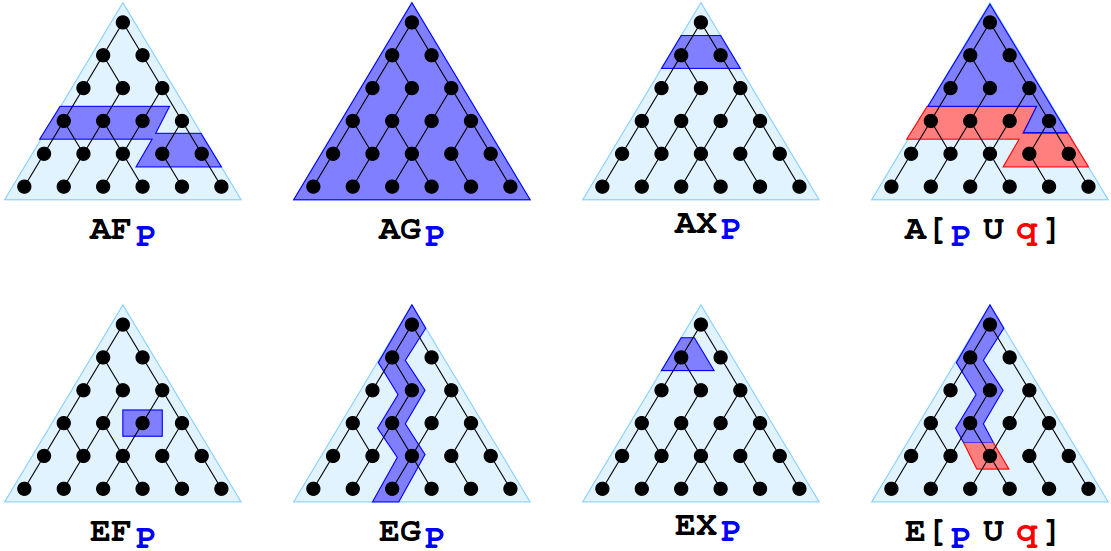
\includegraphics[scale=0.3]{images/tree_examples.png}
    \end{figure}
\end{frame}
\begin{frame}{Semantics}
	\framesubtitle{Definition of model}
	\begin{definition}
		Let $Atoms$ be a set of atomic formulas. A \alert{transition system} or \alert{model} $\M$ is a triple $\M = (S, \to, L)$ in which $S$ is a set of states, $\to$ is a binary relation over $S$ ($\to \subseteq S\times S$) such that for every state $s\in S$, exists a $s'$ that $s \to s'$ and $L: S \to \mathcal{P}(Atoms)$ (or $L: S \to (Atoms \to \{0,1\})$) is a labelling function.
	\end{definition}\pause
    CTL formulas are satisfied by a transition system and a specific state.
    
	{\bf Notation:} we will use $\M,s\vDash \varphi$ to denote that the model $\M,s$ satisfies the formula $\varphi$
\end{frame}

\begin{frame}{Semantics}
    \framesubtitle{Satisfaction}
    \begin{definition}
        The \alert{satisfaction} of a formula in CTL is recursive over the structure of the formula. It can be done as follows:
    \end{definition}
\end{frame}


\begin{frame}{Semantics}
	\framesubtitle{Satisfaction}
	Take an arbitrary model $\M$. Let $s, s_1, s_2, s_3$ be states in $S$. Let $\varphi, \varphi_1, \varphi_2$ be well-formed formulas of CTL. And let $p$ be an atom. The satisfaction of CTL formulas can be defined as follows:
	\begin{itemize}
		\item $\M,s \vDash \top$ and $\M,s \not\vDash \bot$ for all $s \in S$ \pause
		\item $\M,s \vDash p$ iff $p \in L(S)$ \pause
		\item $\M,s \vDash \neg\varphi$ iff $\M,s \not\vDash \varphi$ \pause
		\item $\M,s \vDash \varphi_1 \land \varphi_2$ iff $\M,s \vDash \varphi_1$ AND $\M,s \vDash \varphi_2$ \pause
		\item $\M,s \vDash \varphi_1 \lor \varphi_2$ iff $\M,s \vDash \varphi_1$ OR $\M,s \vDash \varphi_2$ \pause
		\item $\M,s \vDash \varphi_1 \to \varphi_2$ iff $\M,s \not\vDash \varphi_1$ OR $\M,s \vDash \varphi_2$
	\end{itemize}
\end{frame}

\begin{frame}{Semantics}
	\framesubtitle{Satisfaction}
	Take an arbitrary model $\M$. Let $s, s_1, s_2, s_3$ be states in $S$. Let $\varphi, \varphi_1, \varphi_2$ be well-formed formulas of CTL. And let $p$ be an atom. The satisfaction of CTL formulas can be defined as follows:
	\begin{itemize}
		\item $\M,s \vDash \A\X \varphi$ iff for all $s_1$ that $s \to s_1$ and $\M,s_1 \vDash \varphi$. Thus, $\A\X$ says: ``in every next state...''\pause
		\item $\M,s \vDash \E\X \varphi$ iff exists $s_1$ that $s \to s_1$ and $M,s_1 \vDash \varphi$. Thus, $\E\X$ says: ``in some next state...''\pause
		\item $\M,s, \vDash \A\G \varphi$ iff for all paths $s_1 \to s_2 \to s_3 \to ...$ in which $s = s_1$, for all $s_i$, $\M, s_i \vDash \varphi$. Thus, $\A\G$ says: ``In all possible paths from now on in all next states...''\pause
		\item $\M,s, \vDash \A\G \varphi$ iff exists some path $s_1 \to s_2 \to s_3 \to ...$ in which $s = s_1$, for all $s_i$, $\M, s_i \vDash \varphi$ Thus, $\E\G$ says: ``Exists a path from now on in all next states...''
	\end{itemize}
\end{frame}

\begin{frame}{Semantics}
	\framesubtitle{Satisfaction}
	Take an arbitrary model $\M$. Let $s, s_1, s_2, s_3$ be states in $S$. Let $\varphi, \varphi_1, \varphi_2$ be well-formed formulas of CTL. And let $p$ be an atom. The satisfaction of CTL formulas can be defined as follows:
	\begin{itemize}
		\item $\M,s, \vDash \A\F \varphi$ iff for all paths $s_1 \to s_2 \to s_3 \to ...$ in which $s = s_1$, exists $s_i$, $\M, s_i \vDash \varphi$. Thus, $\A\F$ says: ``In all possible paths from now on, in some next state...''\pause
		\item $\M,s, \vDash \E\F \varphi$ iff exists some path $s_1 \to s_2 \to s_3 \to ...$ in which $s = s_1$, that exists $s_i$, $\M, s_i \vDash \varphi$. Thus, $\E\F$ says: ``In some path from now on, in some next state...''\pause
		\item $\M,s, \vDash \A[\varphi_1 \U \varphi_2]$ iff for all paths $s_1 \to s_2 \to s_3 \to ...$ in which $s = s_1$, this path satisfies $\varphi_1 \U \varphi_2$, i.e., exists $s_i$ in the path such that $\M, s_i \vDash \varphi_2$ and, for all $j < i$, $\M, s_j \vDash \varphi_1$. Thus, $\A\U$ says: ``For all paths from now on, until some state...''
	\end{itemize}
\end{frame}
\begin{frame}{Semantics}
    \framesubtitle{Satisfaction}
    Take an arbitrary model $\M$. Let $s, s_1, s_2, s_3$ be states in $S$. Let $\varphi, \varphi_1, \varphi_2$ be well-formed formulas of CTL. And let $p$ be an atom. The satisfaction of CTL formulas can be defined as follows:
    \begin{itemize}
        \item $\M,s, \vDash \E[\varphi_1 \U \varphi_2]$ iff exists some path $s_1 \to s_2 \to s_3 \to ...$ in which $s = s_1$, this path satisfies $\varphi_1 \U \varphi_2$. Thus, $\E\U$ says: ``In some path from now on, until some state...''
    \end{itemize}
\end{frame}